%!TeX root = 4-ml.tex
\documentclass[main]{subfiles}

\begin{document}

\chapter{Statistical Learning of Adsorption Properties}
\vspace*{-1\baselineskip}

\section{Machine Learning Models}

In the field of nanoporous material study, machine learning (ML) models have been widely used to characterize various properties such as adsorption, transport, catalytic or mechanical properties. These models offer a means to replace time-consuming simulations with simpler calculations of key descriptors, thereby aiding in the prediction of desired properties. In other cases, they are used to describe the structure-property relationships learned by the ML model. However, it should be noted that machine learning cannot be considered as a silver bullet since its application requires a comprehensive understanding of the key variables that improves prediction accuracy. In this study, a machine learning model will be built to characterize the separation of xenon from krypton at ambient pressure, utilizing the work on thermodynamic descriptors and knowledge on the effect of pressure on selectivity from the previous chapters.

\subsection{From algorithm to machine learning}

To understand the learning process of machines, it is necessary to understand how computers perform tasks. The human operator plays a key role in this process by designing the solution based on theoretical considerations and creating a list of instructions, known as an algorithm, which outlines the required actions for the computer to achieve the desired outcome under specific circumstances. In the context of physical or chemical science, these algorithms typically articulate the different components of a theoretical model, such as solving equations without analytical solutions or expressions, and addressing probabilistic problems. The previous chapters presented such algorithms used for simulating adsorption processes. For instance, GCMC simulations are based on the statistical physics of phase equilibrium between a gas phase and an adsorption phase within a nanoporous material, and Monte Carlo models are used to replicate the statistics associated with the grand canonical ensemble. Energy sampling algorithms, along with the Widom insertion are additional examples illustrating how computers assist theoreticians in modeling systems under specific chemical and physical conditions.

Machine learning models are also based on algorithms, but their objective differs significantly from that of the above-mentioned examples --- they don't aim at providing comprehensive computational details based on established theoretical principles. As their name suggests, machine learning algorithms aim to learn underlying relationships within input data, enabling them to perform tasks autonomously. The machine learning (ML) algorithm serves as a set of instructions guiding the machine learning process. For instance, clustering algorithms can distinguish different classes of elements within a disordered dataset, leading to the emergence of new concepts. This type of machine learning algorithm is referred to as unsupervised learning, as the data is not pre-labeled, and the machine assists in uncovering the underlying structure. As unsupervised learning extends beyond the scope of this thesis, further details on this algorithm type will not be provided.  it is worth mentioning that supervised learning models are the focus of study, which learn the relationship between labeled data and the characteristics (features or descriptors) of a given dataset. Subsequently, these models can predict the label of unlabeled data based on their characteristics.

The focus of this thesis lies on the supervised learning model, which learns the relationship between labels and their characteristics (referred to as features or descriptors) from a given set of labeled data points, enabling the prediction of labels for unlabeled data based on their characteristics. As an example, predicting tomorrow's weather could involve using past weather data from similar dates to infer whether it will rain. The ML model's features comprise the weather history, while the target variable or label of the data corresponds to the future weather.

The distinctions between a standard algorithm and an ML algorithm can be illustrated by a fascinating board game called Go. This game is traditionally played by two players on a 19$\times$19 board, where each player places bblack/white pieces to gain control over the maximum number of boxes. Based on these simple rules, different algorithms have been developed to make computers play the game. The first Go program was written in the late ’60s to mimic the pattern recognition of Go players when estimating the ``score'' through an influence function,\autocite{zobrist1970feature} and from the ’80s to the beginning of the 21\ex{st} century the first Go programs capable of playing were released. These programs were based on simple alpha-beta search algorithms that sought to test every possible move (while pruning the less promising ones). While they worked well in other games like chess (IBM's Deep(er) Blue beat the world chess champion in 1995), these types of programs in Go were only at the level of a novice player. The difference in performance lies in the combinatorics of both games. Chess has a number of legal positions lower than $10^{47}$,\autocite{website_labelle} while Go has approximately $10^{171}$ legal positions.\autocite{Tromp_2007,github_tromp_go} The state space to explore in Go is incomparably greater, and an increase in computing power that improved the performance of chess-playing computers would not make a significant difference for Go. A drastic reduction in the space to be explored is required for a computer program to work. The biggest improvement came in 2007 when a Monte Carlo tree search was introduced by Couloms.\autocite{Coulom_2007} This algorithm uses heuristics to distinguish between good and bad moves based on human perception of the game. A probability of selection is assigned to the moves according to their potential (policy), and potential moves are randomly selected based on this probability. The average outcomes associated with a parent move provide the value of the move. The computer Go is now more efficient in evaluating moves using a Monte Carlo sampling, and it can now play with average amateur players although it is nowhere near surpassing them. Up until now, the algorithms have been based on human knowledge that the programmer implements directly in the computer using machine instructions. Statistics and randomness are used to guide the machine towards the best moves and reduce their predictability, but the statistics that identify the moves are based on human heuristics that are usually not generalizable. The revolutionary aspect brought about by machine learning in the field aims to improve the evaluation of these statistics using data from previously played games. By using a dataset of 30 million moves, Alpha Go is based on the same Monte Carlo tree search framework, but the formulas behind the probability of searching a move are replaced by a machine learning model called the ``policy network'' and the evaluation of confidence in winning a position is done by a value ``network''.\autocite{Silver_2016} Alpha Go became the first computer program to beat a world champion in 2016. One year later, an improved version called Alpha Go Zero generated its own data by playing games against itself to train a similar machine learning structure as the one presented before. This new version beat the former version 100 times out of 100,\autocite{Silver_2017} marking a new era of computer dominance in Go over the world's best players, with the defeat of another top player further confirming the advent of this new era.

This example showed how the value of each move was learned by the machine through the compilation of knowledge from large datasets in a deep neural network. The main difference between conventional approaches to algorithmic and machine learning is very well illustrated in the previous example. The objective is not to instruct the computer on how to play using player knowledge implemented in formulas and explicit instructions. Instead, an explicit framework with flexible parameters is provided to the model, which needs to learn these parameters using a database. In other words, the model's parameters are adjusted to match the values of a database while having the ability to generalize to situations outside of the database (further discussion on the notion of generalizability will be presented in the following sections). The purpose of this section is not to provide a comprehensive overview of all existing models, but rather to introduce the main concepts of ML through the example of the model used in this thesis for the prediction of selectivity performance.

\subsection{Introduction to supervised learning}

In this thesis, the focus will be on the most common way to statistically learn from data, which is known as supervised learning. As previously introduced, supervised learning entails the extraction of a relationship between the labels of a set of data points and some of their known characteristics or features. This relationship can be referred to as the model or the predictor and is expected to generalize to similar but unseen data. In this section, the goal of the learning algorithm will be formalized when provided with a set of labeled data, to introduce more complex notions in machine learning, such as the bias--variance tradeoff, as well as more specific models used in this chapter like the tree-based models. Various books have been consulted to develop this section, primarily the Elements of Statistical Learning\autocite{Hastie_2009} and an Introduction to machine learning (in French) from Azencott\autocite{azencott2022introduction}.

\subsubsection{Theoretical considerations}

In supervised learning, the algorithm learns from a set of data denoted as $\mathcal{D}_{n}=\left\{(\mathbf{x}_{1},y_{1}),...,(\mathbf{x}_{n},y_{n})\right\}$ with $n$ observed data points, where $\mathbf{x}_{i}$ represents an input observable, which is a vector of $\mathbb{R}^{p}$ ($p=1$ for scalars), and $y_{i}$ represents the label of the data point $i$ that belongs to a set $\mathcal{Y}$ (numerical, categorical or vectorial). 
The observed characteristics can be modeled by a random variable $X$, while the label is represented by another random variable $Y$. The dataset provides only a partial view of the joint probability (see equation~\ref{eq:joint_proba}), and the objective is to generalize the relationship to unseen data. $(X,Y)$ represents all possible combinations of seen and unseen data points.
\begin{equation}\label{eq:joint_proba}
  \forall\ \mathbf{x}\in\mathbb{R}^{p},\ y\in\mathcal{Y},\ \mathbb{P}\left(X=\mathbf{x}, Y=y\right) = \mathbb{P}(X=\mathbf{x})\mathbb{P}(Y=y|X=\mathbf{x})
\end{equation}
The challenge of supervised learning is that a complete picture of the probability law is not provided by the available data. The objective is to determine the most probable label $y$ for a given data point characterized by $\mathbf{x}$, which involves determining the conditional expectation $\E{Y|X=\mathbf{x}}$ of $Y$ given the observable $\mathbf{x}$. This determination relies on the conditional probabilities $\mathbb{P}(Y=y_i|X=\mathbf{x}_j)$ observed across all data points $i,j\in\{1,\ldots,n\}$.

\begin{figure}[ht]
  \centering
    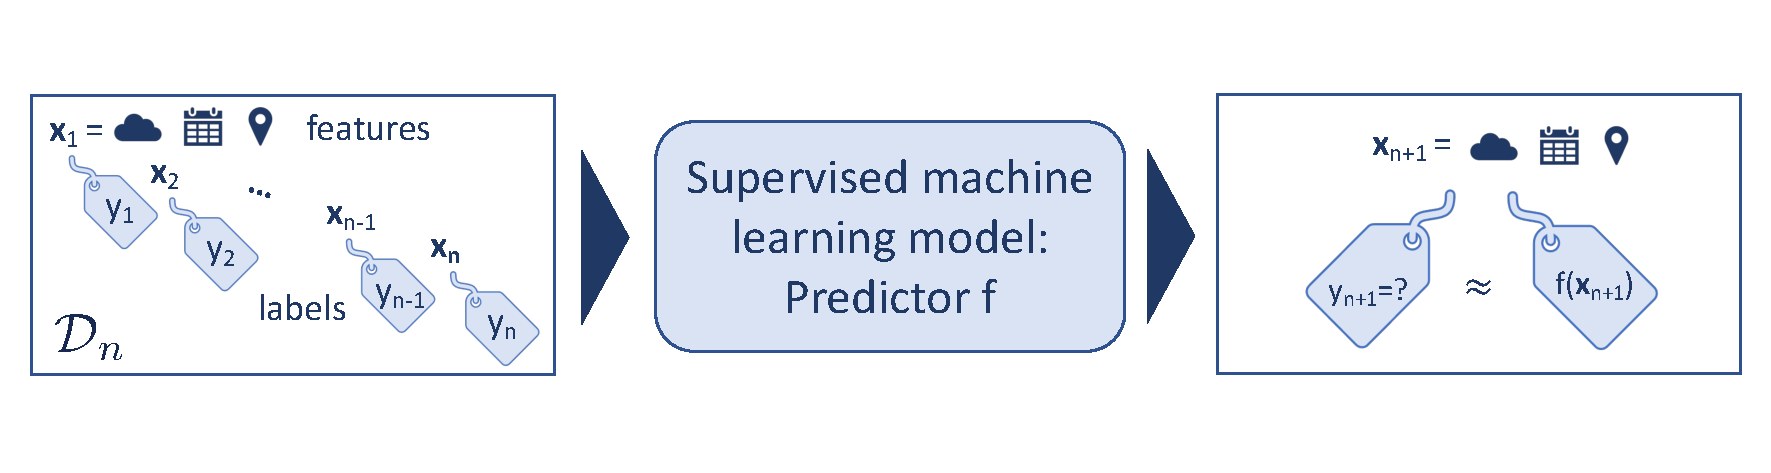
\includegraphics[width=0.9\textwidth]{figures/4-ml/machine learning.pdf}
    \caption{Illustration of the core principle of supervised learning.}\label{fgr:supervised_leaning}
\end{figure}

To achieve this, the learning algorithm uses a ``predictor'' $f$, which can be defined as the function that associates values (features) from $\mathcal{X}=\mathbb{R}^{p}$ with values from $\mathcal{Y}$. By changing the learning model (subsection~\ref{sct:model}) or the feature space $\mathcal{X}$, different domains $\mathcal{F}\subseteq{\mathcal{Y}}^{\mathcal{X}}$ where the prediction function $f$ is sought, can be defined. The domain $\mathcal{F}$ can be either too restrictive, resulting in the found optimal function being far from the theoretical one, or too large, making the optimization problem nearly impossible to solve or leading to a solution that is too close to the data. These issues raise questions regarding fitting, which will be discussed later.

This predictor can be interpreted as the function that provides the most probable outcome $y$ for a given input $\mathbf{x}$. To assess the quality of the predictor, a loss function $\mathcal{L}:\mathcal{Y}\times\mathcal{Y} \rightarrow \mathbb{R}^{p}$ is introduced to compare the predicted value $f(\mathbf{x})$ with the true value $y$ on available dataset $\mathcal{D}_{n}$. The loss function should increase when $f(\mathbf{x})$ deviates from $y$. To extend the definition of the loss to the entire possible space, the theoretical risk $\mathcal{R}$ of a predictor $h$ is introduced using the random variables $X$ and $Y$, such that $\mathcal{R}(h) = \E{\mathcal{L}\left(h(X),Y\right)}$. However, since the exact mapping of the random variables is unknown, the empirical risk $\mathcal{R}_n$ on the known dataset $\mathcal{D}_{n}$ is evaluated istead:
\begin{equation}\label{eq:risk}
  \mathcal{R}_n(h) = \frac{1}{n}\sum_{i=1}^n \mathcal{L}\left(h(\mathbf{x}_i),y_i\right)
\end{equation}

The goal, therefore, is to find a function that minimizes the risk function across the known data, and the optimal predictor $f^*$ can be defined as follows:
\begin{equation}\label{eq:min_f}
  f_n^* = \underset{f\in\mathcal{F}}{\text{arg min}} \mathcal{R}_n(f)
\end{equation}


The risk function can utilize various loss functions, with an increasing emphasis on large errors depending on their definitions. For instance, a quadratic cost function highly penalizes outliers, thus prioritizing a few medium errors over a single large error. Conversely, an absolute cost function does not exhibit this behavior. Since regression models were exclusively utilized in this thesis work, the details of classification loss functions will not be discussed extensively. Instead, the focus will be on regression loss functions. The quadratic loss or squared error loss $\mathcal{L}\e{SE}(f(\mathbf{x}),y)=0.5{\left(y-f(\mathbf{x})\right)}^2$ of a predictor $f$ on a data point $(\mathbf{x},y)$ is simply defined as the squared difference between the prediction and the true label. The multiplicative $0.5$ coefficient is included to simplify the derivatives. This loss is similar to the mean squared error (MSE) used to compare two quantities across a dataset, where the risk function corresponds to half of the MSE on the predictions $\mathcal{D}_n$:
\begin{equation}
  \mathcal{R}\e{SE}(f) = 0.5\frac{1}{n}\sum_{i=1}^n {\left(y_i-f(\mathbf{x}_i)\right)}^2
\end{equation}

A second commonly used loss function is the absolute loss, which is associated with the mean absolute error (MAE) utilized in error evaluation. The loss can be expressed as $\mathcal{L}\e{AE}(f(\mathbf{x}),y)=\left|y-f(\mathbf{x})\right|$, and the risk function associated with it is simply the MAE across the dataset predictions:
\begin{equation}
  \mathcal{R}\e{AE}(f) = \frac{1}{n}\sum_{i=1}^n \left|y_i-f(\mathbf{x}_i)\right|
\end{equation}
It is also possible to introduce a parameter $\epsilon$ to flatten loss function flatter near the minimal error. The $\epsilon$-insensitive loss corresponds to a modified absolute loss $\mathcal{L}_{\epsilon}(f(\mathbf{x}),y)=\max\left(0,\left|y-f(\mathbf{x})\right|\right)$.

Lastly, a Huber loss can be used to combine the less outlier-sensitive absolute loss with the smoothness of the quadratic loss near the minimal error domain. For a given $\delta$, the Huber loss is defined as:
\begin{equation}
  \mathcal{L}_{\delta}(f(\mathbf{x}),y) = \left\{
    \begin{array}{ll}
        \tfrac{1}{2}{\left(y-f(\mathbf{x})\right)}^2 & \mbox{for } \left|y-f(\mathbf{x})\right| \leq \delta \\
        \delta\left(\left|y-f(\mathbf{x})\right| - \tfrac{1}{2}\delta\right) & \mbox{otherwise.}
    \end{array}
  \right.
\end{equation}
A risk function $\mathcal{R}_{\delta}$ can also be determined using this loss function. The Huber loss is considered a robust loss function since it is less sensitive to the outliers (high values of error) and has a very smooth gradient near low error values like the squared error. It can be viewed as a combination of the advantages of both the absolute and squared errors as illustrated on Figure~\ref{fgr:loss_comp}.

\begin{figure}[ht]
  \centering
    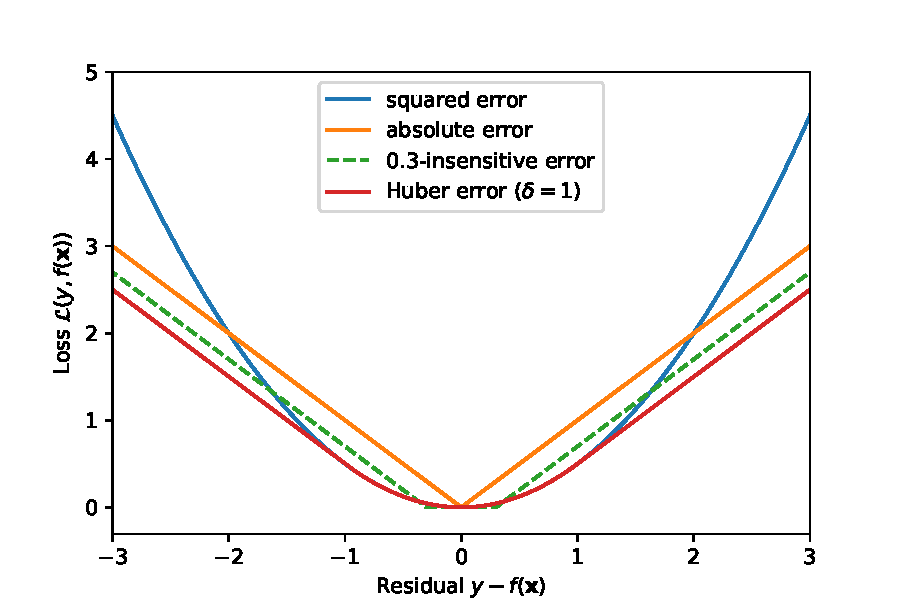
\includegraphics[width=0.6\textwidth]{figures/4-ml/loss_comparison.pdf}
    \caption{Comparison of different loss functions (quadratic loss, absolute loss, $\epsilon$-insensitive and the Huber loss). }\label{fgr:loss_comp}
\end{figure}

Through these theoretical considerations, the process of machine learning from data can hopefully be demystified by formulating this learning process as the optimization of a cost function, which is a common tool in any scientific field. However, this optimization problem poses challenges in the sense that the variable is a function that exists in a high-dimensional space, necessitating approximations to reduce the space. This is why most engineering breakthroughs occur in the conception of the architecture of the ML model, which defines the form of the prediction function $f$. Another difficulty in machine learning is dealing with an ill-posed problem, where one of the three conditions of Hadamard is not satisfied. These conditions pertain to the existence and unicity of a solution and its continuity with respect to the initial conditions. Typically, this issue is addressed through regularization techniques, such as the one introduced by Tikhonov in the second half of the 20\e{th} century. Furthermore, the minimization of the empirical risk does not always align with the minimization of the more global risk (considering all possible observations). In other words, minimizing $\mathcal{R}_n$ does not always yield the same solution as the minimization of $\mathcal{R}$. Therefore, the complexity of the risk optimization problem depends on the chosen loss function and the domain $\mathcal{F}$ defined by the model. Different techniques can be used to construct a solution without without any guarantees of its optimality. One of the biggest challenges in ML is overcoming the problem of generalizability, which will be the topic of the next discussion. 


\subsubsection{Generalization and overfitting}

As previously discussed, the optimization problem is ill-defined and there is no guarantee the model will work on other data points as $n$ goes toward infinite. The generalizability of model consists of ensuring the predictability of unseen data, where the solution does not only correspond to the minimal risk for the data $\mathcal{D}_{n}$ but also for other $m$ data points $\left\{(\mathbf{x}_{n+1},y_{n+1}),\ldots,(\mathbf{x}_{n+m},y_{n+m})\right\}$, all different from the previous set. One of the main phenomena that explain this discrepancy between the solution $f_n^*$ and the ideal solution $f^*$ (considering an infinite amount of data) is the noise in the dataset. The data is not perfectly measured, and the uncertainty attached to each $\mathbf{x}_i$ and $y_i$ values can create a residual noise that needs to be ignored in the learning process. Moreover, the $p$ explanatory variables considered are sometimes not sufficient to model the target phenomenon. To train a generalizable model, it is necessary to ensure sufficient learning to capture the inner relation between $X$ and $Y$ while avoiding fitting the data too closely and capturing the noise along the way. Otherwise, it is said that the model overfits the data. If the model is highly inaccurate even on the training data, it is said to underfit, generally indicating that the model is too simplistic (not enough features or too low-level architecture). 

This problem of overfitting can be summarized in the fundamental notion of bias--variance tradeoff in machine learning and, more generally, in statistics. The error can be broken down in two types: the bias error measures the error made on the available data $\mathcal{D}_n$, while the variance error measures the sensitivity to small variations in the input values. A high bias error corresponds to underfitting, indicating that not enough is learned from the data. A high variance error corresponds to overfitting, indicating too much is learned, even including superfluous relations. To formalize these errors, reference can be made to the empiric risk function $\mathcal{R}_n(f)$ that models the error of the predictor $f\in\mathcal{F}$. To ascertain whether the ideal optimum has been achieved, a comparison with the minimal risk attainable by a predictor possessing infinite knowledge is necessary. This minimal risk is denoted as $\mathcal{R}^* = \underset{\scriptscriptstyle h\in\mathcal{Y}^{\mathcal{X}}} {\text{min}}\mathcal{R}(h)$. This excess error $\mathcal{R}_n(f)-\mathcal{R}^*$ can then be decomposed into two errors, which can be interpreted as the bias and the variance errors:
\begin{equation}\label{eq:generalization_error}
  \mathcal{R}_n(f)-\mathcal{R}^* = \left[\mathcal{R}_n(f) - \underset{\scriptstyle h\in\mathcal{F}} {\text{min}}\mathcal{R}_n(h)\right] + \left[\underset{\scriptstyle h\in\mathcal{F}} {\text{min}}\mathcal{R}_n(h) -\mathcal{R}^*\right]
\end{equation}
